\section{Overview of \vtkm}

%\assign{Hank, editting pass (perhaps trimming)}

The \vtkm library~\cite{Moreland2016} began via a research project funding
from the 
Advanced Scientific Computer Research program within the Office of Science of the
United States Department of Energy.
The goal of the project was to enable scientific visualization on emerging HPC systems via
two approaches:
(1) serving as a repository for interoperable scientific visualization algorithms well suited to accelerator architectures and (2) providing a framework that simplifies the development of visualization algorithms that can be ported across many accelerator devices.

%\ken{Idea from Jay: summarize the filters and stuff we have done in a table so that people can easily add their work.}

%\jay{Table is added and we might simplify this paragraph a little bit and put detailed references into the table.}

At the onset of ECP, \vtkm contained only the most common operations for scientific visualization: contour, threshold, external faces, basic surface simplification, and rendering.
Although this initial set is useful, practitioners almost always require more functionality.
ECP enabled this additional functionality to grow with the introduction of many more algorithms as well as performance improvements to the existing ones.
Table~\ref{tab:algorithms} contains a summary of algorithms provided by \vtkm.
These added features provided the necessary functionality for the tools and applications, discussed later in this paper, that utilized \vtkm to execute on Exascale machines and similar hardware.

%% \begin{figure}[htb]
%%   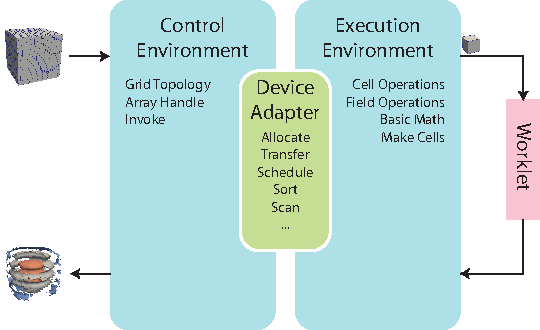
\includegraphics[width=\linewidth]{vtkm-framework}
%%   \caption{The basic \vtkm framework for device portability. \hank{Do we have a copyright issue with using this image?  Has it appeared before?} \ken{I'm not totally sure. For now, let's delete it and use something else instead.}}
%%   \label{fig:vtkm-framework}
%% \end{figure}

%The basic structure for \vtkm's framework is shown in Figure~\ref{fig:vtkm-framework}.
The basic workflow for an algorithm in \vtkm's framework is shown in Figure~\ref{fig:vtkm-workflow}.
%\vtkm provides a framework designed for optimizing both developer time and execution time on
%diverse many-core devices.
The framework separates code into two environments: control and execution.
These correspond to the ``host'' and ``device,'' respectively, in a GPU development environment.
This separation is maintained even when 
there is not a clear separation between host and device, which is the case for some accelerators such as the Xeon Phi~\cite{Jeffers2016}.
%This design promotes developer efficiency, as
%\vtkm simplifies implementations for current and future algorithms, and also provides 
%automatic and efficient porting of these algorithms across different devices.


To achieve portability, \vtkm contains a device adapter that manages interaction with a variety of devices.
The entirety of \vtkm can be ported with a change to the device adapter.
%
Further, all execution code (``device code'') is implemented with standard C++14,
%and thus universal for any GPU device.
and thus can be compiled for any device supporting the C++ language.
\hank{Is this statement too strong?}
\ken{I've qualified the statement to be more accurate. I am leaving out some qualifications about using only the subset of the language supported by the device compiler, but would that much detail be necessary here?}

\vtkm uses multiple approaches to achieve efficient parallelization.
One approach is 
to enable data to be divided in small pieces for parallel execution
using a 
flexible data model~\cite{Meredith2012}.
A second approach is 
to utilize
data parallel primitive methods~\cite{Blelloch1990}.
Data parallel primitives allow algorithms to be implemented as a sequence of data parallel operations, such as scan, sort, or reduce.
Early work explored how to implement scientific visualization using data parellel primitives~\cite{Lo2012}.
To simplify the implementation further, \vtkm provides ``meta'' data parallel primitives~\cite{Moreland2021} that incorporate common patterns for scientific data that were demonstrated to be efficient.
Finally, note the \vtkm design achieves developer efficiency --- 
streamlined algorithm development as well as 
automatic
porting to new architectures with an efficient implementation 
